\item Se o segmento $CD$ tem uma velocidade angular $\omega_{CD}=\SI{6}{\radian/\second}$, determine a velocidade do ponto $E$ no segmento $BC$ e a velocidade angular do segmento $AB$ no instante mostrado.

\import{../answers/}{answer-8}

\vspace{-2.2cm}
\begin{flushright}
	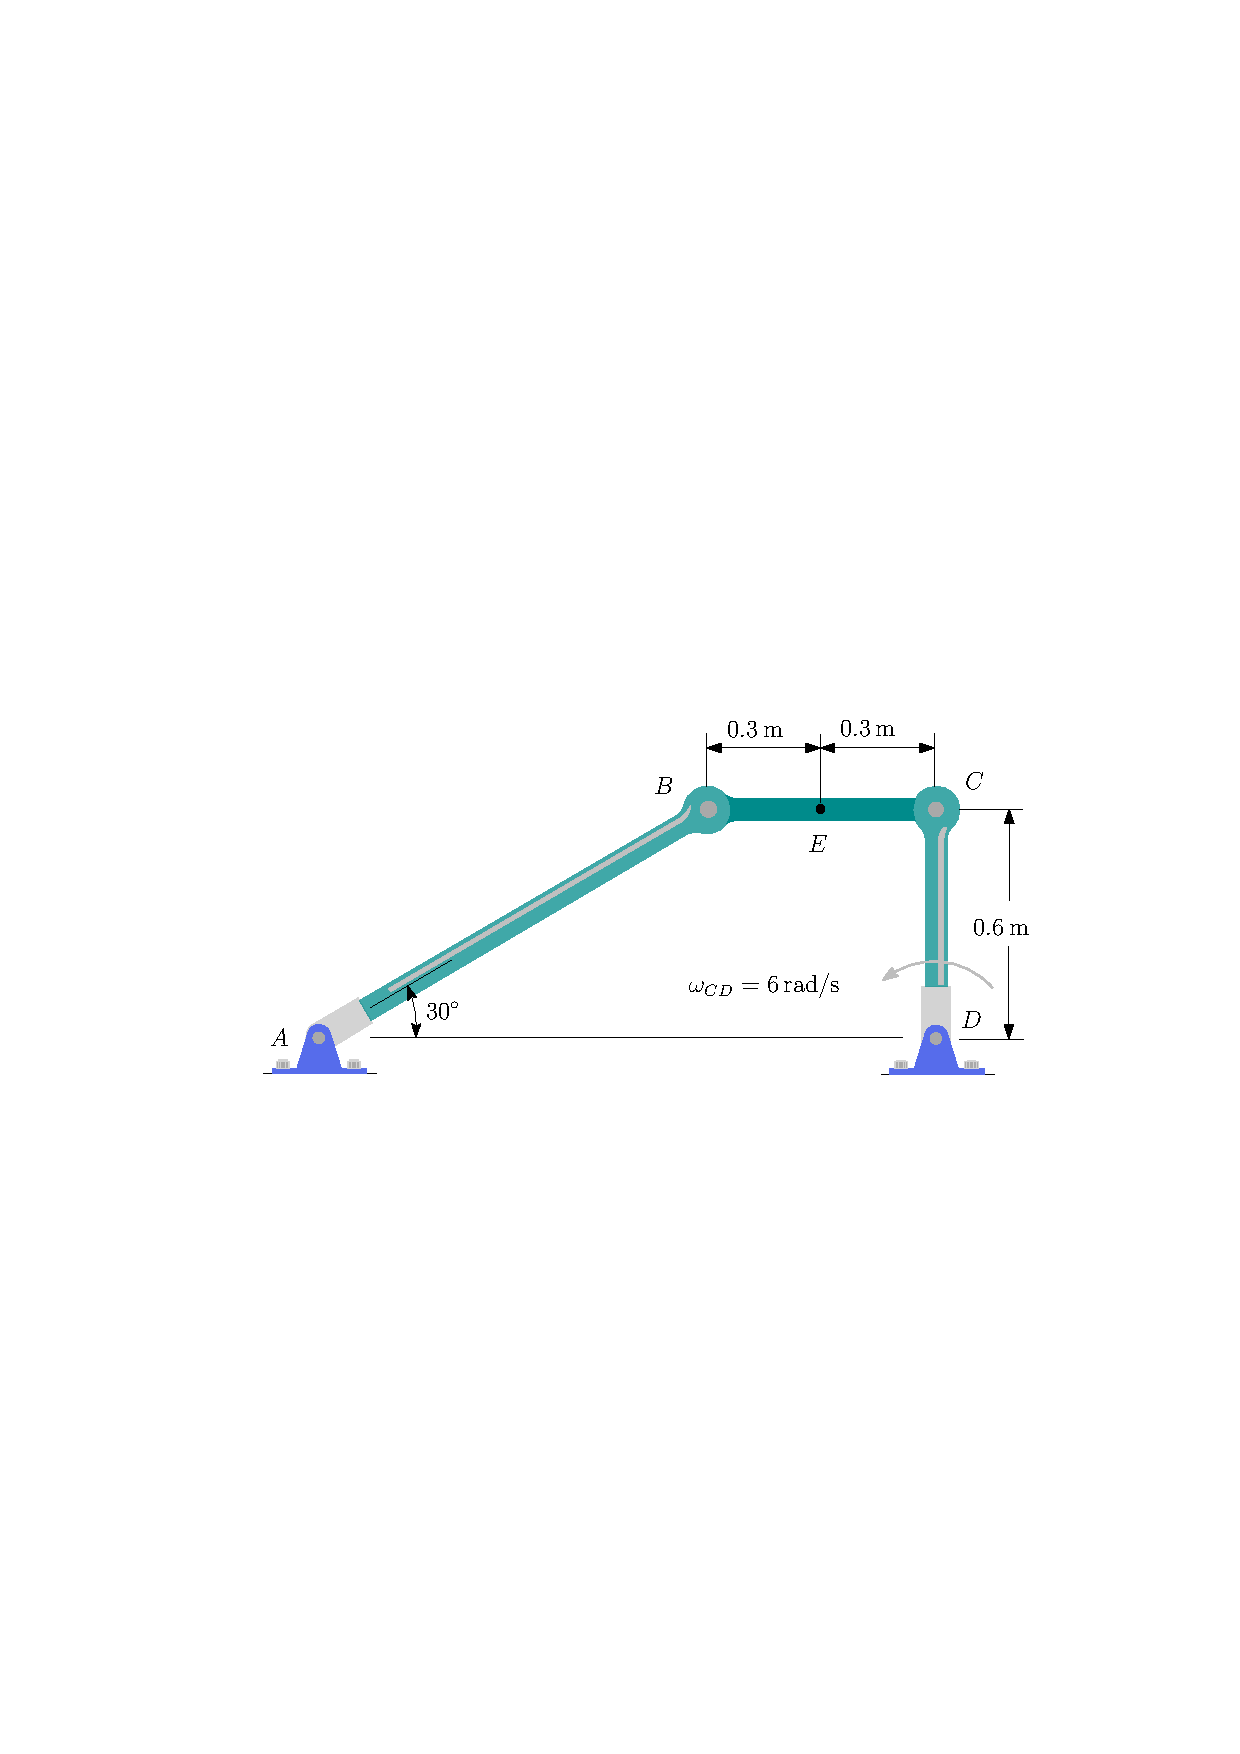
\includegraphics[scale=1]{images/draw_10}
\end{flushright}